%
% File proposal_template.tex
%
%% Based on the style files for ACL 2018, NAACL 2018/19, which were
%% Based on the style files for ACL-2015, with some improvements
%%  taken from the NAACL-2016 style
%% Based on the style files for ACL-2014, which were, in turn,
%% based on ACL-2013, ACL-2012, ACL-2011, ACL-2010, ACL-IJCNLP-2009,
%% EACL-2009, IJCNLP-2008...
%% Based on the style files for EACL 2006 by 
%%e.agirre@ehu.es or Sergi.Balari@uab.es
%% and that of ACL 08 by Joakim Nivre and Noah Smith

\documentclass[11pt,a4paper]{article}
\usepackage[hyperref]{acl2019}
\usepackage{times}
\usepackage{latexsym}
\usepackage{enumitem}
\usepackage{url}
\usepackage[utf8]{inputenc}
\usepackage{amsmath} % Add the necessary package for the control sequence
\usepackage{setspace} % Add the necessary package for adjusting line spacing
\usepackage{hyperref}
% \usepackage{subcaption}
% Required packages (add to preamble)
\usepackage{listings}
\usepackage{xcolor}
\usepackage{enumitem}
\usepackage{booktabs}
\usepackage{hyperref}
\usepackage{url}
\usepackage{graphicx}
\usepackage{subcaption}
\aclfinalcopy % Uncomment this line for the final submission
%\def\aclpaperid{***} %  Enter the acl Paper ID here

%\setlength\titlebox{5cm}
% You can expand the titlebox if you need extra space
% to show all the authors. Please do not make the titlebox
% smaller than 5cm (the original size); we will check this
% in the camera-ready version and ask you to change it back.

\newcommand\BibTeX{B\textsc{ib}\TeX}

\title{PyLinguist: Automated Translation of Python for Hindi Programmers}

\author{First Author \\
  Antara Tewary\\ 
  G01413546\\
  \texttt{atewary@gmu.edu} \\\And
  Second Author \\
  Ankit Kumar\\ 
  G01436204\\
  \texttt{akumar37@gmu.edu}\\\And
  Third Author \\
  Homa Haghighi\\ 
  G01436204\\
  \texttt{akumar37@gmu.edu}}

\date{December 6,2024}

\begin{document}
\maketitle

\section{Introduction}
Python is a popular programming language, which has gained its popularity due to many factors, which include its readability and intuitive English-like syntax that makes the code accessible to English speakers. However, this can be a significant barrier for non-English speakers who have to grapple with both the programming concepts and learning a new language. Our project addresses this issue by developing a comprehensive translation system that converts Python code from English to Hindi, making Python programming more accessible to Hindi speakers while maintaining code functionality and readability.
            \subsection{Task / Research Question Description} 
            Core research questions are-\\
            - How can we effectively translate Python's syntax, keywords, and natural language elements while preserving code functionality?\\
            - What combination of translation techniques provides optimal results for code translation??\\
            - How can we quantitatively and qualitatively evaluate the effectiveness of code translation?\\ \\
            Our project implements a three-stage translation pipeline combining keyword dictionaries, Google Translate API, and GPT models, with comprehensive evaluation metrics to assess translation quality and code functionality preservation.
            \subsection{Motivation \& Limitations of existing work} 
            While Python's pseudo-code nature simplifies programming for English speakers, it presents significant challenges for non-English speakers who comprise the majority of the global population. Research has shown that students learn programming concepts more effectively when using a coding language based on their native language. Current solutions like CodeInternational partially address this issue by translating comments and identifiers, but they fall short of providing a complete solution that encompasses Python's built-in functions, keywords, and error messages.\\ \\ 
            Limitations of existing work include:
            \begin{itemize}[itemsep=0pt, topsep=0pt]
                \item Incomplete coverage of Python's language elements
                \item Lack of consistency in technical term translation
                \item Limited handling of language-specific challenges
                \item Insufficient preservation of code functionality
                \item Absence of comprehensive evaluation metrics
            \end{itemize} 
            \subsection{Proposed Approach} 
            We propose a three-stage pipeline for translating Python code between English and Hindi while preserving functionality. Stage 0 involves preprocessing Python code from the Hugging Face dataset to extract clean samples. In Stage 1, we use a combination of rule-based translation with a keyword dictionary and the Google Translate API, where a KeywordManager maps Python keywords and a CodeTranslator handles compound words, comments, and strings. Stage 2 refines the translations using GPT-4o Mini, which enhances the initial translations through example-based learning. This hybrid approach leverages precise keyword mapping, neural machine translation for natural language, and contextual enhancement via GPT, ensuring reliable and functional translations.
            
            \subsection{Likely challenges and mitigations} 
            There are several challenges in trying to translate Python code between English and Hindi. Our implementation tackles these through specific mitigation strategies:-
            \begin{itemize}[itemsep=0pt, topsep=0pt]
              \item \textbf{Compound Word Translation}: Code often contains compound words separated by underscores. The \texttt{translate\_token} method in the \texttt{CodeTranslator} class handles this by splitting compound words, translating individual components, and rejoining them with underscores to maintain code readability.
              \item \textbf{Code Structure Preservation}: Maintaining code formatting and structure is crucial for readability and execution. The \texttt{translate\_line} method preserves indentation and line structure by measuring leading whitespace before translation and restoring it afterward.
              \item \textbf{Translation Reliability}: To handle potential translation failures, we apply two important features in our code. The \texttt{safe\_translate} method, which includes a retry mechanism for failed translations. Next is the \texttt{CheckpointManager} class which maintains translation progress. This allows longer translation tasks to be resumed if they are interrupted.
              \item \textbf{Keyword Translation}: Python keywords and built-in functions need consistent translation. The \texttt{KeywordManager} class maintains a dictionary mapping between English and Hindi keywords, which use Joshua Otten's curated dataset \cite{otten-etal-23-unipy}.
              \item \textbf{Comments and String Handling}: Code comments need a different handling than executable code. The \texttt{translate\_line} method identifies comments by looking at the \texttt{'\#'} character and applying separate translation rules for code and comment sections. This preserves the comments. 
            \end{itemize}
            These challenges are addressed through specific implementation, though future work can definitely improve these solutions.

\section{Related Work}
\begin{itemize}
  \item \cite{otten-etal-23-unipy}
  
  This paper introduced the PyLinguist framework to address the challenges of making Python accessible to non-English speakers. Their work demonstrates that Python's pseudo-code nature, while beneficial for English speakers, creates barriers for others who must master both programming concepts and English simultaneously. They propose automatically translating Python's natural language elements (keywords, error messages, identifiers) into other human languages. Their preliminary implementation enables coding in 5 additional languages and provides a roadmap for developing automated translation frameworks. Our work builds upon their vision by implementing a specific English-Hindi translation pipeline that combines rule-based translation with neural methods.
  \item \cite{Piech2019HumanLI}
  
  This paper introduces CodeInternational, a tool designed to translate code comments and identifiers across multiple human languages, helping non-English speakers learn programming more easily. The study emphasizes the importance of making code accessible in native languages but primarily focuses on Java and comments/identifiers. Our project differs by aiming to translate the entire Python syntax, not just comments or identifiers, providing a more comprehensive solution for Python programming education in non-English languages.
  
  \item \cite{10.5555/2819009.2819097}. 
  
  This paper explores how code, like natural language, follows repetitive patterns, which can be modeled using statistical language models such as n-grams. The work applies these models to tasks like code completion and suggests that programming languages are predictable. While this research focuses on enhancing software development efficiency, our project applies similar language models but aims to address the language accessibility challenge by translating Python syntax for non-English speakers. 
  
  \item \cite{10.1145/3196398.3196402}
  
  The authors demonstrate the application of deep learning models to analyze software repositories and improve tasks like bug prediction and code completion. Their deep learning models perform well on large software corpora. Our project builds on these deep learning concepts but uses them to handle the translation of Python's structure and syntax into multiple human languages, a task that extends beyond improving code completion. 
  
  \item \cite{10.1109/ASE56229.2023.00076}
  
  UniXcoder proposes a model that utilizes code comments and abstract syntax trees (AST) to improve code representation and generation across different programming tasks. This work focuses on enhancing programming tasks like code completion through multi-modal data. In contrast, our project focuses on the translation of Python's syntax into human languages, leveraging multi-modal data like AST for language translation and accessibility rather than improving programming performance. 
\end{itemize}

\section {Methodology}
\subsection{Pipeline Overview}
approach for translating Python code between English and Hindi consists of three main stages: data preprocessing, initial translation, and GPT-based enhancement. Each stage builds upon the previous one, ensuring quality translations while preserving code functionality.
\subsubsection{Stage 0: Data Preprocessing}
The dataset that we use is the python-code-dataset-500k from Hugging Face \cite{jtatman2021python}. We load this dataset using Hugging Face datasets library. We first clean the dataset by removing unnecessary columns, like 'instruction' and 'system', to focus on the code content.\\ 

The main part of our preprocessing involves extracting clean Python code from the dataset. We implement this using a regex pattern to extract the code enclosed within these tags. The regex patterns ensure that we capture only the actual python code while removing any surrounding markup or documentation. After extraction, we perform a cleaning step using \texttt{dropna()} to remove any entires that might have been corrupted or imporperly formatted while we did the extraction process.\\ 

The preprocessed dataset is stored in a structured CSV format with an \texttt{'English\_code'} column. The final processed dataset contains 67,063 total entries, of which 25,549 are unique code samples.\\ 

To manage the processed data, we create a directory system. We have a \texttt{data} directory, where we maintain separate files for different evaluation configurations, specifically creating distinct files for experiments with 5, 10, 20, and 30 examples (translations\_gpt\_10r\_5e.csv through translations\_gpt\_10r\_30e.csv).

\subsubsection{Stage 1: Initial Translation}
 This stage implements several interconnected steps that work together to perform basic English to Hindi code translation.\\

 They \texttt{KeywordManager} class hangles the python-specific translations. It reads from a predefined \texttt{Joshua\_Keywords.csv}, which contains 234 English-Hindi keyword pairs curated by Joshua Otten \cite{otten2023unipy}. This csv file contains other languages too, but since we focus on English to Hindi translation, we remove all non-Hindi translation columns and create a dictionary that maps English keywords to their Hindi equivalents. This class also implements special case handling for single-letter variable names commonly used in Python programming, specifically mapping -
 \begin{figure}
    \centering
    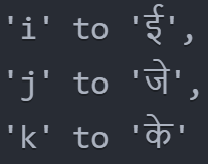
\includegraphics[width=0.15\textwidth]{Images/ijk-mappings.png}
    \caption{Translation Mapping Overview}
    \label{fig:translation_system}
\end{figure}
\texttt{CodeTranslator} class handles the translation of words by first splitting them at underscore (\_). translating each component individually, then rejoining them with (\_). It also takes care of space that might be introduced during translation.\\ 

\texttt{safe\_translate} method implements a retry mechanism that attempts each transaction upto three times. If a transaction fails after al retries, it returns the original text rather than failing completely, ensuring that the translation process does not stop abruptly.\\ 

\texttt{translate\_line} method handles the code structure by preserving and measuring the indentation of each line. It also separates code and comments, denoted by \texttt{\#}, and applies different translation rules to each section.\\

To manage the translation process, we use the \texttt{CheckpointManager} class, which maintains the translation progress. This allows us to resume longer translation tasks if they are interrupted.\\

\subsubsection{Stage 2: GPT-based Enhancement}
The second stage uses GPT-4o mini model \cite{gpt4omini} to refine and improve the output from Stage 1. \texttt{GPTTranslator} class uses previously translated examples which serve as a reference material for the model. We use 5,10,20 0r 30 examples to study the impact of example quantity on the translation quality.\\ 

The \texttt{create\_prompt} creates carefully formatted prompts for the GPT model (Appendix \ref{sec:appendix}). Each prompt contains three key sections: example translations showing the desired transformation pattern, explicit instructions for maintaining code structure and handling translations, and the partially translated code that needs enhancement. This structured approach helps guide the model toward producing consistent and reliable translations.\\ 

The translation process is done by \texttt{translate\_code} method, which applied they keyword replacement strategy from Stage 1, then creates an appropriate prompt for GPT 4o Mini. The model runs with tempaerature 0 to maximize the consistency in output.
\subsection{Evaluation Framework}
\subsubsection{Dataset and Test Configuration}
\begin{itemize}[itemsep=0pt, topsep=0pt]
    \item \textbf{Total Dataset}: 500k Python code samples from hugging face \cite{jtatman2021python}
    \item \textbf{Test Configuration}:\\ 
    - Translation set: 10 samples selected for translation\\
    - Example sets: Varying sizes (5,10,20,30) that are given to GPT model for reference\\ 
    - Human evaluation set: 20 samples evaluated by human evaluators
    \item \textbf{Keyword Dictionary}: 234 pre-mapped English-Hindi keyword pairs translated by Joshua Otten.
\end{itemize}
\subsubsection{Human Evaluation Framework}
Two bilingual evaluators (Hindi-English) with 4 years of experience in Python programming evaluated 20 code samples generated by our model. They followed the following rating scale-\\ 
\textit{\underline{Rating Scale(1-5)}}:
\begin{itemize}[itemsep=0pt, topsep=0pt]
    \item \textbf{1}: Unusable and incorrect translation
    \item \textbf{2}: Partially correct translation, major revisions needed
    \item \textbf{3}: Mostly correct translation, minor revisions needed
    \item \textbf{4}: Good translations with minimal revisions needed
    \item \textbf{5}: Perfect translation, no revisions needed
\end{itemize}
\textit{\underline{Evaluation Criteria}}:
\begin{itemize}[itemsep=0pt, topsep=0pt]
    \item \textbf{Syntax Correctness (SC)}: Proper keyword translation, code structure preservation and indentation accuracy
    \item \textbf{Semantic Preservation (SP)}: Logic preservation, variable scope maintenance and function behavior consistency
    \item \textbf{Hindi Language Quality (HLQ)}: Evaluating natural hindi expressions, the technical term consistency, comment clarity and code readability
\end{itemize}
\subsubsection{Technical Evaluation Framework}
\textit{\underline{Syntax Validation}}
\begin{itemize}[itemsep=0pt, topsep=0pt]
    \item \textbf{AST(Abstract Syntax Tree) Validation}: Tests if translated code produces valid Python AST and gives a binary outcome of Valid/Invalid
    \item \textbf{Token Structure Analysis}: Compares token types between original and translated code, uses Python's tokenize module
\end{itemize}
\textit{\underline{Semantic Testing}}\\We use the \texttt{SemanticTester} class to text the following:
\begin{itemize}[itemsep=0pt, topsep=0pt]
    \item \textbf{Execution Equivalence}:Runs both original and translated code, compares outputs for identical inputs
    \item \textbf{Runtime Behavior}: Tests error handling, verifies output types and memory usage patterns
\end{itemize}
\textit{\underline{Translation Quality Metrics}}
\begin{itemize}
  \item \textbf{BLEU Score Evaluation}: Compares the translated code with the original code using BLEU score.
  \item \textbf{Back Translation Validation}: Translates the translated code back to English and compares it with the original code. We use the same Pipeline as the main translation task, but in reverse.
\end{itemize}
\section{Experiments}

\subsection{Datasets}
\begin{itemize}[itemsep=0pt, topsep=0pt]
    \item \textbf{Primary Code Dataset}:\\ 
    - \underline{Name}: python-code-dataset-500k\\
    - \underline{Source}: Hugging Face \cite{jtatman2021python}\\
    - \underline{Access}: Public dataset, accessed via Hugging Face datasets library\\
    - \underline{Usage in code}: for extracting Python code examples from \texttt{output} column
    - underline{Preprocessing}: We extract the python code enclosed in the \texttt{<pythoncode>} tags using regex\\ 
    - \underline{Dataset split}: No specific tran/dev/test splits implemented
    \item \textbf{Keyword Dataset}:\\
    - \underline{Name}: Joshua\_Keyword.csv\\
    - \underline{Content}: 234 English-Hindi keyword pairs\\
    - \underline{Usage in code}: for direct translation of Python keywords\\
    - \underline{Preprocessing}: Curated by Joshua Otten \cite{otten-etal-23-unipy}\\
    - \underline{Access}: Local file, obtained from \cite{otten2023unipy}
\end{itemize}

\subsection{Implementation} 
Our implementation builds upon the Universal Python framework proposed by \cite{otten2023unipy}. We use the Hugging Face \cite{jtatman2021python} for training and Google Translate API \cite{googletranslateapi} and GPT-4o Mini \cite{gpt4omini} for translation. The keyword mapping dictionary is taken from Otten's work \cite{otten-etal-23-unipy} on multi-lingual python translation.\\ \\ 
\textbf{Link to our repository}:\href{https://github.com/StringAna/PyLinguist/blob/main/code_trials/Project.ipynb}{PyLinguist Code}

\section{Results}
\subsection{Discussion}
Our evaluation of the Python-to-Hindi translation system yielded consistent performance across different configurations, as shown in \ref{tab:translation-results} and visualized in Fig. \ref{fig:metrics-analysis}(a), with all metrics maintaining scores above 0.65. The violin plots in Fig.  \ref{fig:metrics-analysis}(b) reveal the distribution characteristics of our evaluation metrics, showing wider variation in BLEU scores compared to more tightly clustered semantic and overall scores, while maintaining consistent median values across configurations. The semantic similarity analysis, depicted in the heatmap in Fig. \ref{fig:syntax-and-semantic-analysis}(a), demonstrates robust performance with mean scores ranging from 0.907 to 0.937, maximum scores consistently reaching 1.0, and low standard deviations between 0.111 and 0.209. Fig. \ref{fig:syntax-and-semantic-analysis} illustrates the syntax validation results, showing near-perfect syntax validity across all configurations, with only the 20-example configuration showing a slight 0.1\% invalid syntax rate while all other configurations maintained 100\% validity. This comprehensive evaluation, supported by both the tabulated results in \ref{tab:translation-results} and the visual representations across all four figures, indicates strong and stable performance of our translation system, particularly in maintaining semantic similarity and syntactic correctness across different example counts.
\begin{table}[htbp]
    \small  % Makes the font slightly smaller to fit
    \centering
    \caption{Translation Quality Results Across Different Example Counts}
    \begin{tabular}{|l|c|c|c|c|}
    \hline
    \textbf{Metrics} & \textbf{5 Ex.} & \textbf{10 Ex.} & \textbf{20 Ex.} & \textbf{30 Ex.} \\
    \hline
    BLEU Score & 0.7150 & 0.7035 & 0.6860 & 0.7357 \\
    \hline
    Syntax Valid Rate & 1.0000 & 1.0000 & 0.9000 & 1.0000 \\
    \hline
    Semantic Similarity & 0.9296 & 0.9370 & 0.8662 & 0.9070 \\
    \hline
    Overall Score & 0.8815 & 0.8802 & 0.8174 & 0.8809 \\
    \hline
    \end{tabular}
    \label{tab:translation-results}
    \end{table}

\begin{figure}[!t]
    \centering
    \begin{minipage}{0.95\columnwidth}
        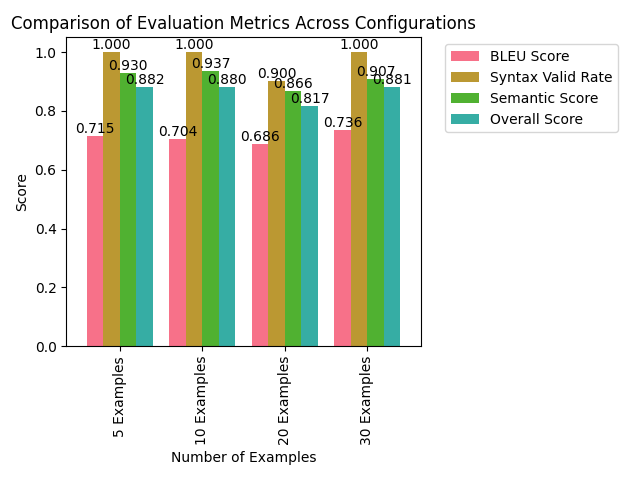
\includegraphics[width=1.1\linewidth,height=6cm,keepaspectratio]{Graphs/overall_metrics_comparison.png}
        \vspace{-0.2cm}
        \caption*{(a) Overall Metrics Comparison}
        \label{fig:overall-metrics-comparison}
    \end{minipage}
    \vspace{0.1cm}
    
    \begin{minipage}{0.95\columnwidth}
        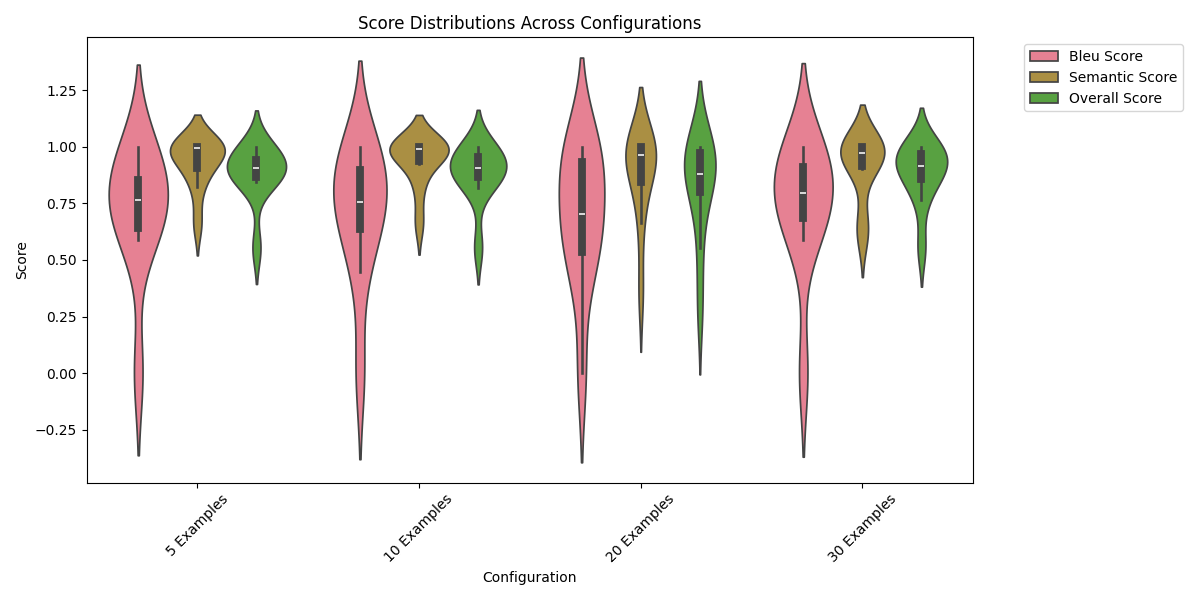
\includegraphics[width=1.1\linewidth,height=10cm,keepaspectratio]{Graphs/score_distributions.png}
        \vspace{-0.2cm}
        \caption*{(b) Score Distributions}
    \end{minipage}
    \vspace{-0.2cm}
    \caption{Performance Metrics Analysis}
    \label{fig:metrics-analysis}
\end{figure}

\begin{figure}[!t]
    \centering
    \begin{minipage}{0.95\columnwidth}
        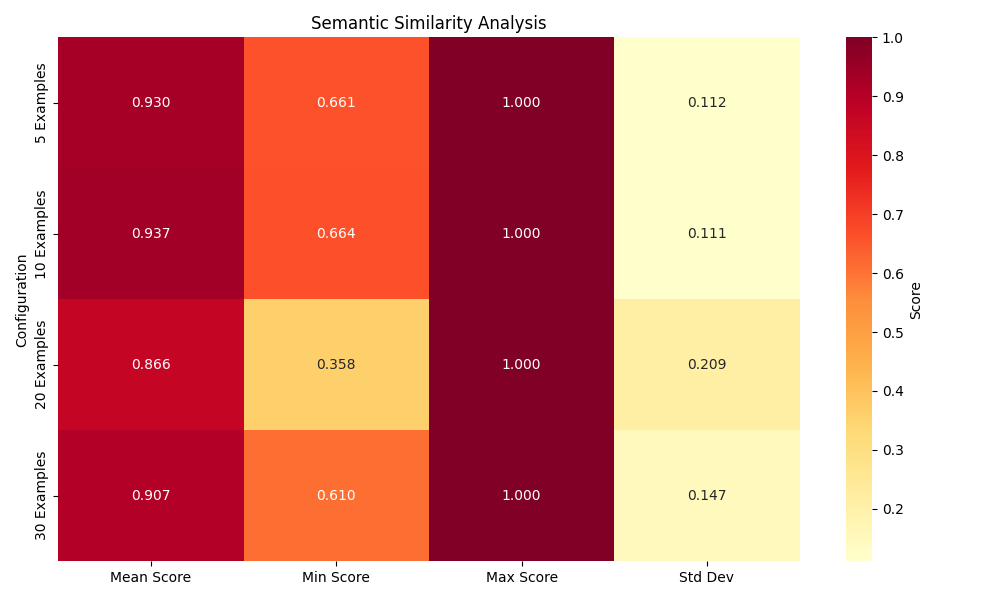
\includegraphics[width=\linewidth,height=4cm,keepaspectratio]{Graphs/semantic_similarity_heatmap.png}
        \vspace{-0.2cm}
        \caption*{(a) Semantic Similarity Heatmap}
    \end{minipage}
    \vspace{0.1cm}
    
    \begin{minipage}{0.95\columnwidth}
        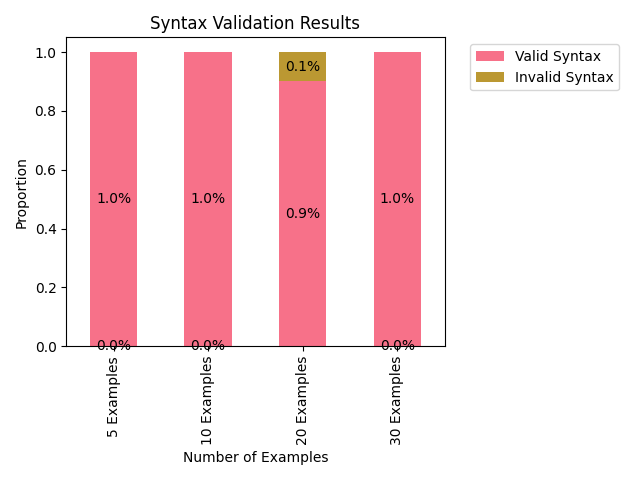
\includegraphics[width=\linewidth,height=6cm,keepaspectratio]{Graphs/syntax_analysis.png}
        \vspace{-0.2cm}
        \caption*{(b) Syntax Analysis}
    \end{minipage}
    \vspace{-0.2cm}
    \caption{Syntax and Semantic Analysis}
    \label{fig:syntax-and-semantic-analysis}
\end{figure}

\subsection{Resources}
This project was developed using the following resources:
\subsubsection{Computational Resources}
\begin{itemize}[itemsep=0pt, topsep=0pt]
    \item Python environment with standard libraries and specific packages like nltk, transformers, and deep-translator
    \item OpenAI's GPT-4o-mini model for translation enhancement
    \item Local CPU computation
    \item Streamlit for frontend development
\end{itemize}
\subsubsection{Time and Development}
\begin{itemize}[itemsep=0pt, topsep=0pt]
    \item Development Time: 4-5 weeks
    \item Total Development Hours: 120 hours
    \item Development Environment: Jupyter Notebook, VSCode
\end{itemize}

\subsection{Error Analysis}
Our analysis revealed several interesting cases where our translation system both succeeded and failed. Here we discuss key examples to highlight the system's strengths and limitations.
\subsubsection{Failure Cases}
Each of the figures (Figure \ref{fig:failure-cases-1} and \ref{fig:failure-cases-2}) illustrates a different type of failure case, where the translation system struggled to convert a specific code snippet to its contextual Hindi meaning. The pipeline converts it to the Hindi equivalent of the most used english word (string, char, state, etc.) which is not always the correct translation in the context of the code. This leads to a loss of readability in the translated code.
\begin{figure}[!t]
    \centering
    \begin{minipage}{0.95\columnwidth}
        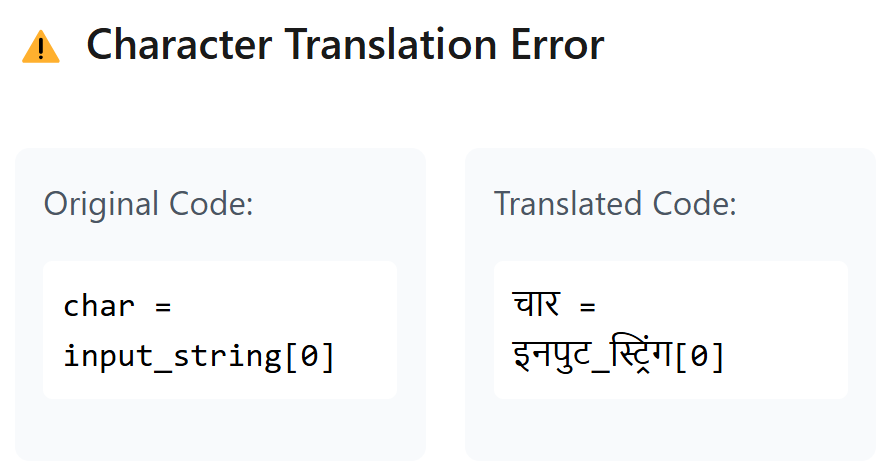
\includegraphics[width=0.7\linewidth,height=4cm,keepaspectratio]{Images/char_translation_error.png}
        \vspace{-0.2cm}
        \caption*{(a) Character Translation Error}
        \label{fig:char-translation-error}
    \end{minipage}
    \vspace{0.1cm}  
    \begin{minipage}{0.95\columnwidth}
        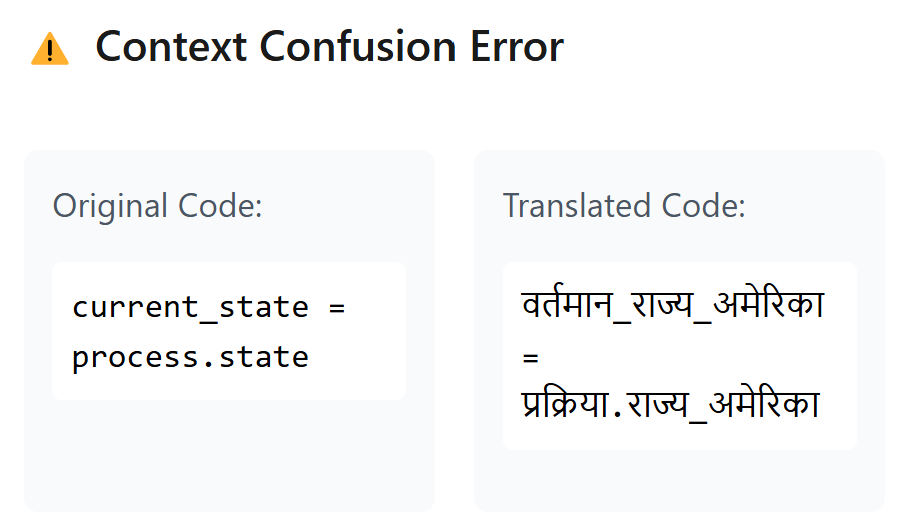
\includegraphics[width=0.7\linewidth,height=4cm,keepaspectratio]{Images/context_confusion_error.png}
        \vspace{-0.2cm}
        \caption*{(b) Context Confusion Error}
        \label{fig:context-confusion-error}
    \end{minipage}
    \vspace{-0.2cm}

    \caption{Failure Cases - 1}
    \label{fig:failure-cases-1}
\end{figure}
\begin{figure}[!t]
\begin{minipage}{0.95\columnwidth}
    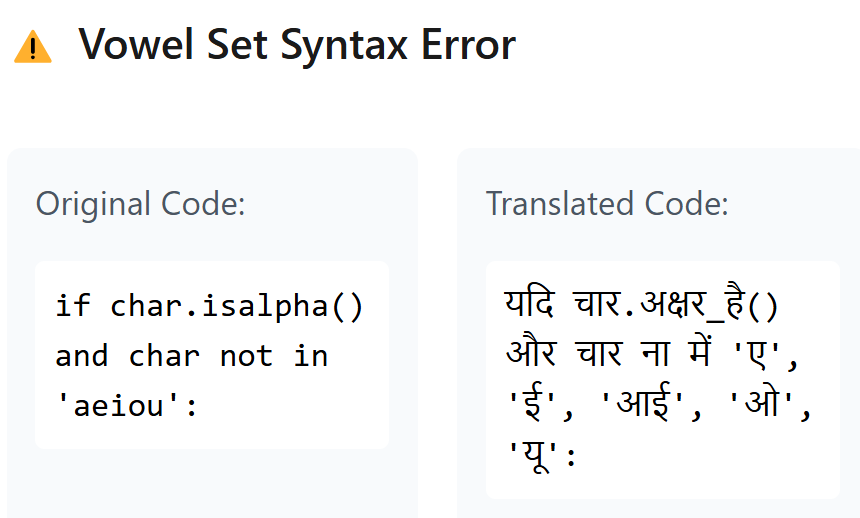
\includegraphics[width=0.7\linewidth,height=4cm,keepaspectratio]{Images/vowel_set_syntax_error.png}
    \vspace{-0.2cm}
    \caption*{(c) Vowel Set Syntax Error}
    \label{fig:vowel-set-syntax-error}
\end{minipage}
\vspace{0.2cm}

\begin{minipage}{0.95\columnwidth}
    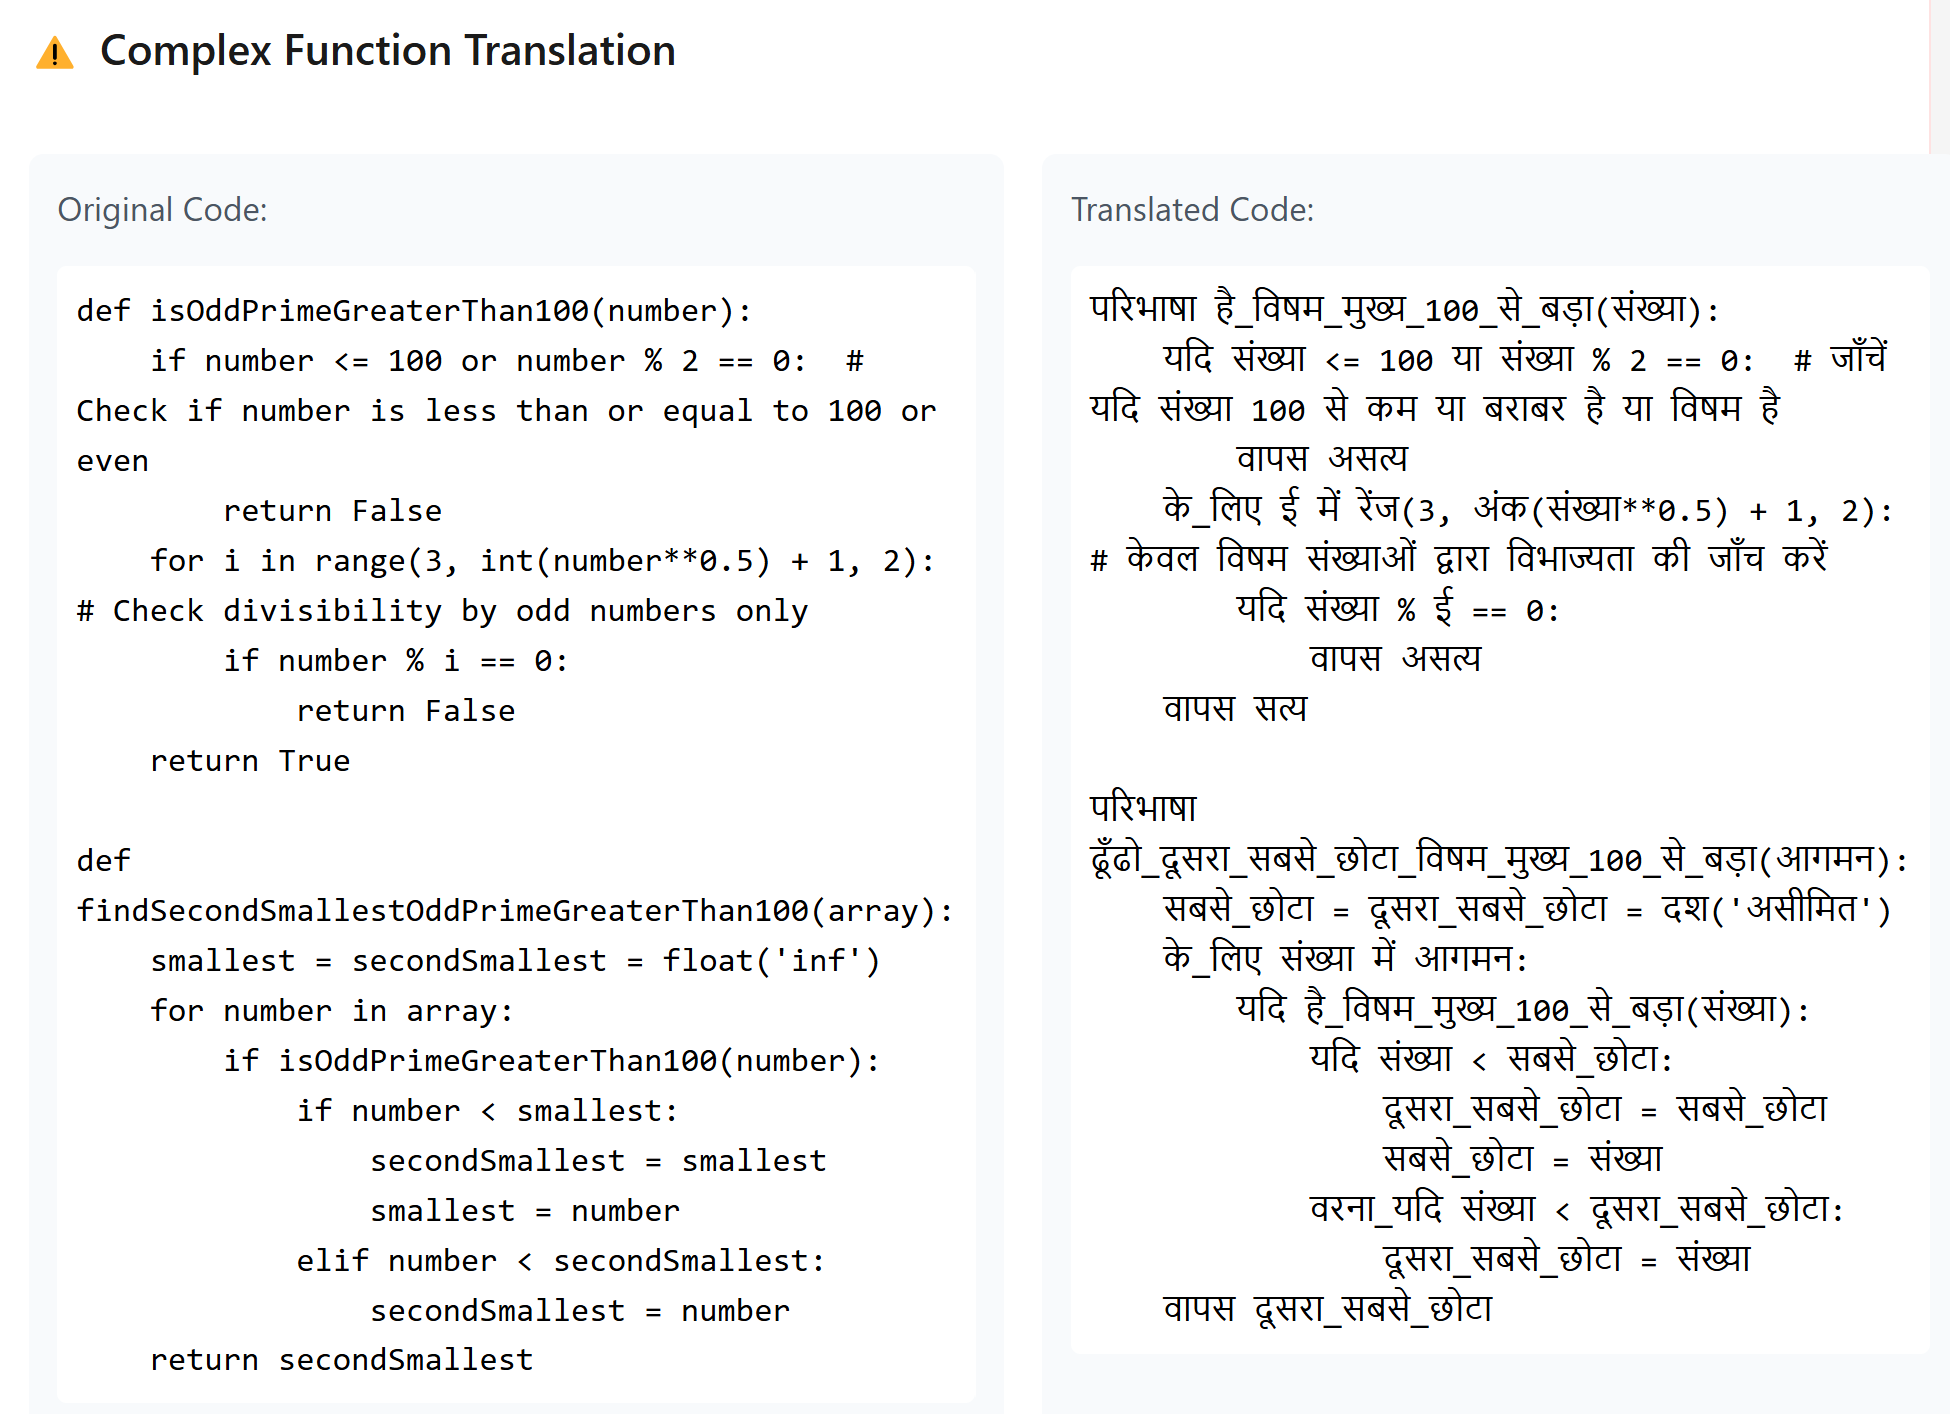
\includegraphics[width=1.1\linewidth,height=8cm,keepaspectratio]{Images/complex-function-translation.png}
    \vspace{-0.2cm}
    \caption*{(d) Complex Function Translation}
    \label{fig:complex-function-translation}
\end{minipage}
\vspace{-0.2cm}
\caption{Failure Cases - 2}
\label{fig:failure-cases-2}
\end{figure}
\begin{figure}
    \centering
    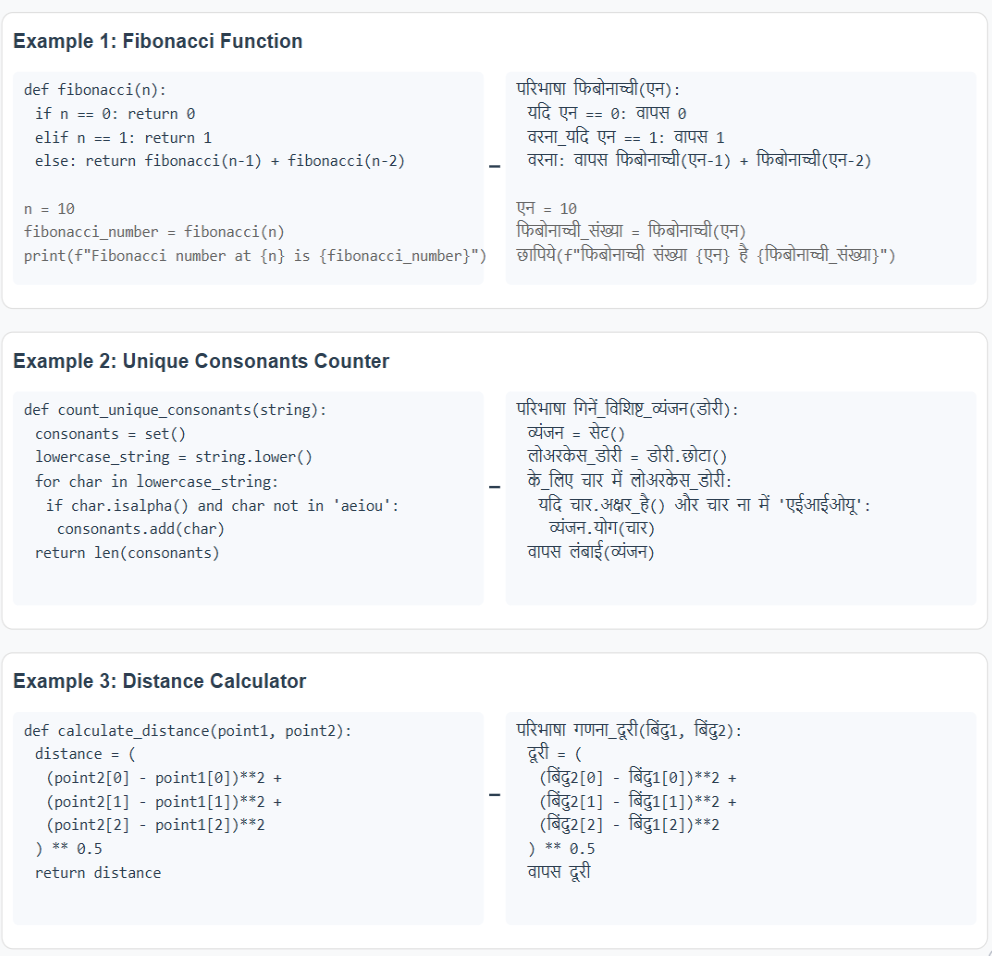
\includegraphics[width=0.9\linewidth,height=7cm,keepaspectratio]{Images/success-cases.png}
    \caption{Success Cases}
    \label{fig:success-cases}
\end{figure}
\subsubsection{Success Cases}
\begin{itemize}[itemsep=0pt, topsep=0pt]
    \item \textbf{Keyword Translation and Syntax Preservation}: The system demonstrated robust performance in maintaining syntactic validity across different configurations. As shown in Table \ref{tab:translation-results}, three out of four configurations achieved a perfect syntax valid rate of 1.0000, with only a slight decrease to 0.9000 for the 20-example configuration. This is further visualized in Figure \ref{fig:syntax-and-semantic-analysis}(b), which illustrates the consistently high syntax validation rates.
    \item \textbf{Semantic Preservation}:The system showed strong capability in preserving the semantic meaning of code during translation. According to Table \ref{tab:translation-results}, semantic similarity scores remained high across all configurations, with the 10-example configuration achieving the highest score of 0.9370. The semantic similarity heatmap in Figure \ref{fig:syntax-and-semantic-analysis}(a) provides a detailed view of this performance, showing consistent results across different metrics including mean scores and standard deviations.
    \item \textbf{Overall Translation Quality}: The system maintained high overall translation quality, as evidenced by the comprehensive metrics shown in Figure \ref{fig:metrics-analysis}(a). The overall scores remained consistently above 0.81 across all configurations, with the 5-example configuration achieving the highest score of 0.8815 (Table \ref{tab:translation-results}). The BLEU scores, while slightly lower, still maintained respectable values ranging from 0.6860 to 0.7357, indicating good translation fidelity.
    The score distributions shown in Figure \ref{fig:metrics-analysis}(b) further support these findings, demonstrating consistent performance across different evaluation metrics and confirming the robustness of our translation system.
\end{itemize}
\section{Robustness Study}
Explain your approach for Evaluating the Model Robustness. Describe what robustness analysis you have performed. Provide sufficient details about your perturbation data, how you created it, how you used it as a robustness benchmark to evaluate the model, in what metrics, etc.

\subsection{Results of Robustness Evaluation}
Describe the evaluation results of your reproduced model on the robustness benchmark that you created. Include at least 2 examples where the model performs well and 2 examples where it fails (i.e., being not robust). Provide sufficient analysis and your thoughts on the observations.

\subsection{Discussion} 
Provide any further discussion here, e.g., what challenges did you face when performing the analysis, and what could have been done if you will have more time on this project? Imagine you are writing this report to future researchers; be sure to include "generalizable insights" (e.g., broadly speaking, any tips or advice you'd like to share for researchers trying to analyze the robustness of an NLP model).

\section{Conclusion}
summarize your contribution in three sentences
\appendix
\label{sec:appendix}
\section{Prompts and Generation Configurations}

\subsection{GPT-4o Mini Configuration}
The following configuration was used for all GPT-4o Mini interactions:

\begin{itemize}
    \item Model: gpt-4o-mini
    \item Temperature: 0
    \item Maximum retries: 3
    \item Response format: Raw code without explanations
\end{itemize}

\subsection{System Prompts}
\subsubsection{Code Translation System Prompt}
The following system prompt was used for the main translation task:
\begin{quote}
``You are a Expert Python code translator who understands the nuanses of language in coding and converts code from English to Hindi code while preserving functionality. Return only the translated code without any explanation.''
\end{quote}

\subsubsection{Back-Translation System Prompt}
For evaluation purposes, the following system prompt was used:
\begin{quote}
``You are a Python code translator converting Hindi code to English.''
\end{quote}

\subsection{User Prompts}
\subsubsection{Main Translation Prompt Template}
This template was used for each translation, with examples and code filled in dynamically:
\begin{quote}
Complete the translation of this partially English Python code to completely Hindi python code:
\begin{itemize}
\item Translate variable names, function names, strings and comments to Hindi
\item Join multi-word Hindi translations with underscores
\item Break down compound English words separated by underscores and translate each part into sensible Hindi and join them back with underscores
\item Preserve code structure and syntax
\end{itemize}

Here are some examples of translations:

[Example 1]:\\
English code:\\
\{original\_code\_1\}\\
Hindi translated code:\\
\{translated\_code\_1\}\\
------------------------

[Example N]:\\
English code:\\
\{original\_code\_n\}\\
Hindi translated code:\\
\{translated\_code\_n\}

Now translate partially translated code to completely in Hindi:\\
\{code\_to\_translate\}
\end{quote}

\subsubsection{Back-Translation Prompt Template}
Used for evaluation through back-translation:
\begin{quote}
Complete the translation of this partially translated Python code to English:
\begin{itemize}
\item The code already has Python keywords translated to English
\item Translate remaining variable names and comments
\item Convert Hindi compound words (with underscores) to appropriate English terms
\item Preserve code structure and syntax
\end{itemize}

Partially translated code:\\
\{partially\_translated\_code\}
\end{quote}

\subsection{Example Configurations}
Four different configurations were tested, varying the number of examples provided to the GPT model for each translation task:

\begin{itemize}
    \item Configuration 1: 5 examples
    \item Configuration 2: 10 examples
    \item Configuration 3: 20 examples
    \item Configuration 4: 30 examples
\end{itemize}


% \section{Credits}

% This document has been adapted from the instructions
% for earlier ACL and NAACL proceedings,
% including 
% those for 
% NAACL 2019 by Stephanie Lukin and Alla Roskovskaya, 
% ACL 2018 by Shay Cohen, Kevin Gimpel, and Wei Lu, 
% NAACL 2018 by Margaret Michell and Stephanie Lukin,
% 2017/2018 (NA)ACL bibtex suggestions from Jason Eisner,
% ACL 2017 by Dan Gildea and Min-Yen Kan, 
% NAACL 2017 by Margaret Mitchell, 
% ACL 2012 by Maggie Li and Michael White, 
% those from ACL 2010 by Jing-Shing Chang and Philipp Koehn, 
% those for ACL 2008 by JohannaD. Moore, Simone Teufel, James Allan, and Sadaoki Furui, 
% those for ACL 2005 by Hwee Tou Ng and Kemal Oflazer, 
% those for ACL 2002 by Eugene Charniak and Dekang Lin, 
% and earlier ACL and EACL formats.
% Those versions were written by several
% people, including John Chen, Henry S. Thompson and Donald
% Walker. Additional elements were taken from the formatting
% instructions of the \emph{International Joint Conference on Artificial
%   Intelligence} and the \emph{Conference on Computer Vision and
%   Pattern Recognition}.

\bibliographystyle{acl_natbib} % We choose the "plain" reference style
\bibliography{refs} % Entries are in the refs.bib file

\end{document}
